\nonstopmode
\documentclass[10pt, a4paper]{article}
\parindent=20pt
\parskip=8pt
\usepackage[width=15.5cm, left=3cm, top=2.5cm, height= 24.5cm]{geometry}
\usepackage[spanish]{babel}
\usepackage[utf8]{inputenc}
\usepackage{fancyhdr}
\usepackage{latexsym}
\usepackage{caratula}
\usepackage{epsfig}
\usepackage{pdfpages}
%\usepackage{algorithmicx}
\usepackage{lastpage}
\usepackage{amsfonts}
\usepackage{listings}
\usepackage{algorithm}
\usepackage{algpseudocode}
\usepackage{pdfpages}
\usepackage{amsmath}
\usepackage{verbatim}
\usepackage{graphicx}
\usepackage{float}
\graphicspath{{imgs/}}

% Acomodo fancyhdr.
\pagestyle{fancy}
\thispagestyle{fancy}
\addtolength{\headheight}{1pt}
\lhead{Teor\'ia de las Comunicaciones}
\rhead{TP1}
\cfoot{\thepage /\pageref{LastPage}}
\renewcommand{\footrulewidth}{0.4pt}
\renewcommand{\thesubsubsection}{\thesubsection.\alph{subsubsection}}


\author{Teor\'ia de las Comunicaciones, DC, UBA.}
\date{}
\title{}

\begin{document}
	
\thispagestyle{empty}
\materia{Teor\'ia de las Comunicaciones}
%\submateria{Trabajo Pr\'actico Nº1}
\titulo{Trabajo Práctico Nº2}
\integrante{Rivero, Maximiliano}{366/07}{maxirivero088@gmail.com}
\integrante{Izcovich, Sabrina}{550/11}{sizcovich@gmail.com}
\integrante{Rogani, Marcos}{520/05}{marcos.rogani@gmail.com}

\maketitle

\tableofcontents
\newpage

\section{Introducción}

En el siguiente trabajo práctico, experimentamos $traceroute$ con herramientas y técnicas frecuentes a nivel de red. Para ello implementamos, en primer lugar, una $tool$ que permitiera realizar un $traceroute$ mediante sucesivos paquetes con TTLs incrementales, calculando los RTTs entre cada salto para los que se recibiría una respuesta ICMP de tipo \textit{time exceeded}. 

Luego, adaptamos la $tool$ realizada para que, una vez terminada la búsqueda, calculara el valor standard o valor Z del RTT (ZRTT) de cada salto $i$ con respecto a la ruta global de la siguiente manera: \\
$$ZRTT_i = \frac{RTT_i - \overline{RTT}}{SRTT}$$\\
siendo $\overline{RTT}$ y $SRTT$ el promedio y el desvío standard de los RTTs de la ruta, respectivamente. Por otra parte, los $RTT_i$ corresponden al tiempo de ida y vuelta dentre el hop $i$ y el hop $i-1$, siendo éstos consecutivos.

Por último, utilizamos la $tool$ para estudiar y analizar rutas a universidades en diferentes lugares del mundo.

Para un análisis adecuado, realizamos gráficos de distribuciones de RTTs estudiando qué saltos son estadísticamente significativos con respecto a la ruta analizada. A partir de esta herramienta, detectamos saltos correspondientes a enlaces submarinos, entre otros. 

\section{Introducción Teórica}
\begin{itemize}
\item \textbf{ICMP(Internet Control Message Protocol):} Protocolo de control que forma parte del núcleo de la arquitectura TCP/IP. El mismo se encarga de proveer mensajes de error y de control. Éstos son:
\begin{itemize}
\item Errores en los datagramas IP.
\item Necesidad de comunicar información de diagnóstico.
\item Necesidad de comunicar información de ruteo.
\end{itemize}
Los paquetes constan de una sección de datos y un header con la siguiente estructura:

\begin{figure}[H] %[h] Aqui [b] para button [t] para top
\begin{center}
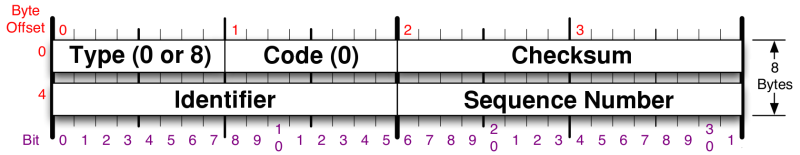
\includegraphics[width=410pt]{../imgs/icmp.png}
\caption{Header de ICMP.}
\end{center}
\end{figure}

\item \textbf{Mensajes de control de ICMP}:
Los mensajes de control que analizaremos a lo largo del trabajo son los siguientes:
\begin{itemize}
\item \textbf{Echo Reply (tipo 0)}: Consiste en un mensaje generado como respuesta a un mensaje Echo Request (petición de Eco).
\item \textbf{Echo Request (tipo 8)}: Consiste en un mensaje de control que se envía a un host con la expectativa de recibir de él un Echo Reply (Respuesta eco).
\item \textbf{Time Exceeded (tipo 11)}: Consiste en un mensaje que se utiliza para indicar que el tiempo de vida de un paquete llegó a su fin.
\end{itemize}

\item \textbf{Round-Trip Time}: Corresponde al retardo del tránsito de paquetes a través de la red IP desde que es enviado hasta volver al emisor, pasando por el destino.

\item \textbf{Traceroute}: Consiste en una herramienta de diagnóstico que muestra la ruta y mide el RTT.
\end{itemize}

\section{Desarrollo}
Para la implementación del traceroute, seguimos el siguiente algoritmo:

\begin{algorithm}
\caption{Algoritmo de Traceroute}
\begin{algorithmic}
\Procedure{traceroute}{$IP_{dst}$}

\State $h\gets IP_{dst}$
\State $ttl\gets 1$
\State $anotadas \gets \{\}$
\Repeat
	\State $h.TTL \gets ttl$
	\State $enviar(h, EchoRequest, TimeOut)$
	\If {$obtener(TimeExceeded)\ \&\&\ \neg obtener(TimeOut)$}
    	\State $anotadas.push(IP_{rcv})$
    \Else
    	\State $anotadas.push(^*)$
    \EndIf
    \State $ttl\gets ttl+1$
\Until{$IP_{dst} = IP_{rcv}$}
\EndProcedure
\end{algorithmic}
\end{algorithm}

donde $h$ representa el host destino e $IP_{rcv}$ representa la IP del hop del que proviene el paquete recibido. Por otro lado, $ttl$ representa el \textit{time to live} del paquete y $TTL$ el campo correspondiente en el header del mismo.

Para la segunda parte del análisis, modificamos la implementación con el fin de que, una vez terminada la búsqueda, calculara el valor standard o valor Z del RTT (ZRTT) de cada salto $i$ con respecto a la ruta global. Para ello, tuvimos en cuenta las siguientes definiciones:\\

\textit{\textbf{Media:}}
$$\overline{x} = \frac{1}{n} \sum_{1=1}^{n}x_i$$


\textit{\textbf{Desvío standard:}}
$$\sigma = \sqrt{\frac{1}{n} \sum_{1=1}^{n}(x_i - \overline{x})^2}$$

El cambio dio como resultado el siguiente algoritmo:

\begin{algorithm}[H]
\caption{Algoritmo de Traceroute con ZRTT}
\begin{algorithmic}
\Procedure{traceroute}{$IP_{dst}$}

\State $h\gets IP_{dst}$
\State $ttl\gets 1$
\State $anotadas \gets \{\}$
\State $RTTs \gets \{\}$
\Repeat
	\State $h.TTL \gets ttl$
	\State $enviar(h, EchoRequest, TimeOut)$
	\State $clock.reset()$
	\If {$obtener(TimeExceeded)\ \&\&\ \neg obtener(TimeOut)$}
    	\State $anotadas.push(IP_{rcv})$
    \Else
    	\State $anotadas.push(^*)$
    \EndIf
    \State $RTTs_i \gets clock.now()$
    \State $ttl\gets ttl+1$
    \State $ZRTT_i \gets \frac{RTTs_i - promedio(RTTs)}{standDesv(RTTs)}$
\Until{$IP_{dst} = IP_{rcv}$}
\EndProcedure
\end{algorithmic}
\end{algorithm}

Las implementaciones se realizaron en python. Para hallar la ubicación de las direcciones IP utilizamos $pygeoip$. Para ello, fue necesario descargar la base de datos $GeoLiteCity$\footnote{https://code.google.com/p/pysnip/downloads/detail?name=GeoLiteCity.dat} que le asigna una ubicación a cada dirección IP.

Por otro lado, para la construcción de gráficos utilizamos $matplotlib$.

Con el fin de que los resultados fueran variados, elegimos como hosts destino los servidores web de tres universidades ubicadas en continentes distintos.
Las universidades utilizadas fueron:
\begin{itemize}
\item \textbf{University of South Africa}: www.unisa.ac.za\\
Esta universidad se encuentra en Sudáfrica, África.
\item \textbf{University of Zurich}: www.uzh.ch\\
Esta universidad se encuentra en Suiza, Europa.
\item \textbf{International University of Japan}: www.iuj.ac.jp\\
Esta universidad se encuentra en Japón, Asia.
\end{itemize}
\newpage
\section{Resultados}
Con el fin de evaluar distintas opciones, decidimos correr el algoritmo de $traceroute$ desde un host utilizando el servicio de \textbf{Fibertel} y desde otro utilizando \textbf{Telefónica}.

En primer lugar, decidimos realizar un gráfico de seguimiento de acuerdo a las $longitudes$ y $latitudes$ resultantes del traceroute. Para ello, corrimos el script trace.py con cada sitio web y con un time to live de 30 (por ser el valor TTL máximo utilizado por defecto). Luego, realizamos los gráficos correspondientes.

Por último, realizamos los gráficos correspondientes a las estadísticas pedidas. Éstas son, para cada hop, RTT promedio (el RTT promedio de todos los paquetes recibidos provenientes de ese hop) y ZRTT. Decidimos agregar un umbral para la identificación de enlaces submarinos según los ZRTT relativos obtenidos para cada enlace. El uso de los ZRTT relativos presenta una manera detallada de identificar variaciones de tiempo entre enlaces, pudiendo identificar nodos con una diferencia de RTT mayor al promedio, como tendría un enlace submarino debido a la distancia que recorren los datos. 

Los resultados obtenidos fueron los que siguen:

\subsection{University of South Africa}

\begin{figure}[H] %[h] Aqui [b] para button [t] para top
\begin{center}
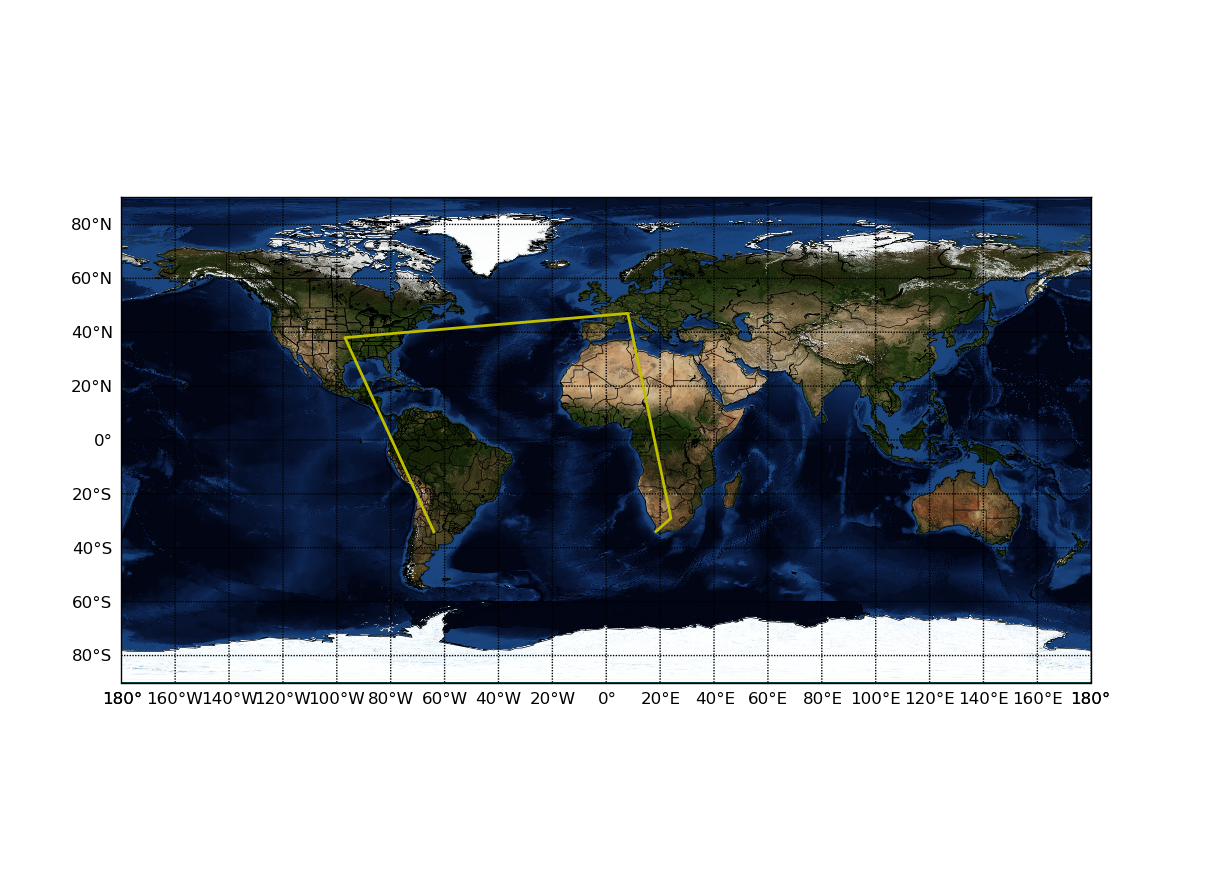
\includegraphics[width=400pt]{../imgs/map-unisa.png}
\caption{Ruta hacia International University of South Africa desde servicio Fibertel.}
\end{center}
\end{figure}

\begin{figure}[H] %[h] Aqui [b] para button [t] para top
\begin{center}
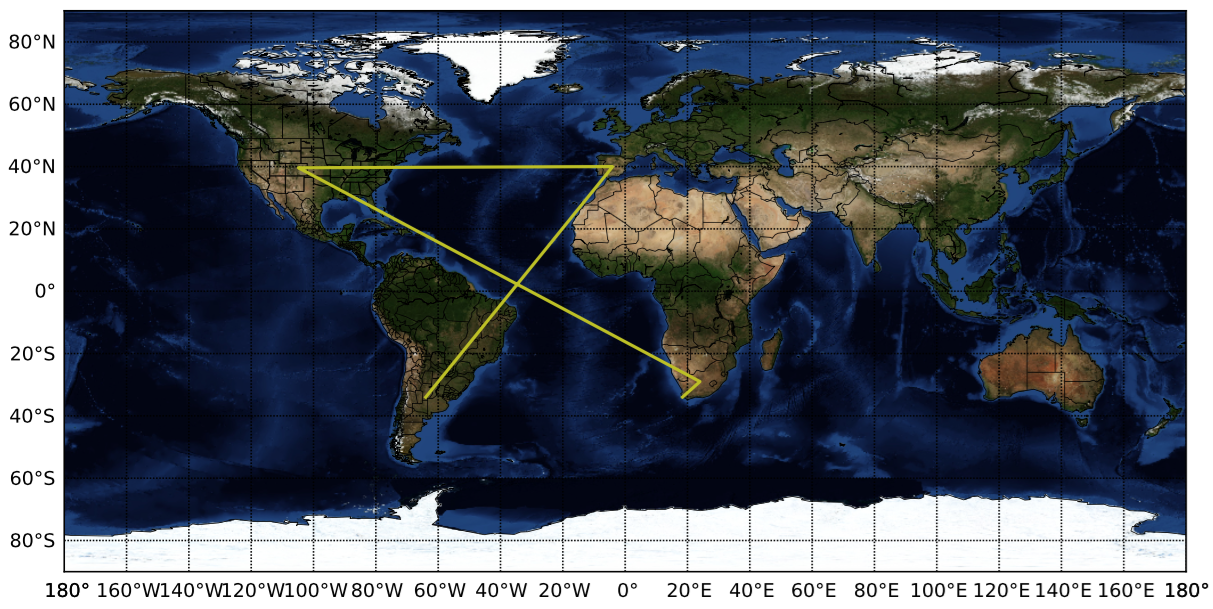
\includegraphics[width=400pt]{../imgs/map-unisa(telef).png}
\caption{Ruta hacia International University of South Africa desde servicio Telefónica.}
\end{center}
\end{figure}

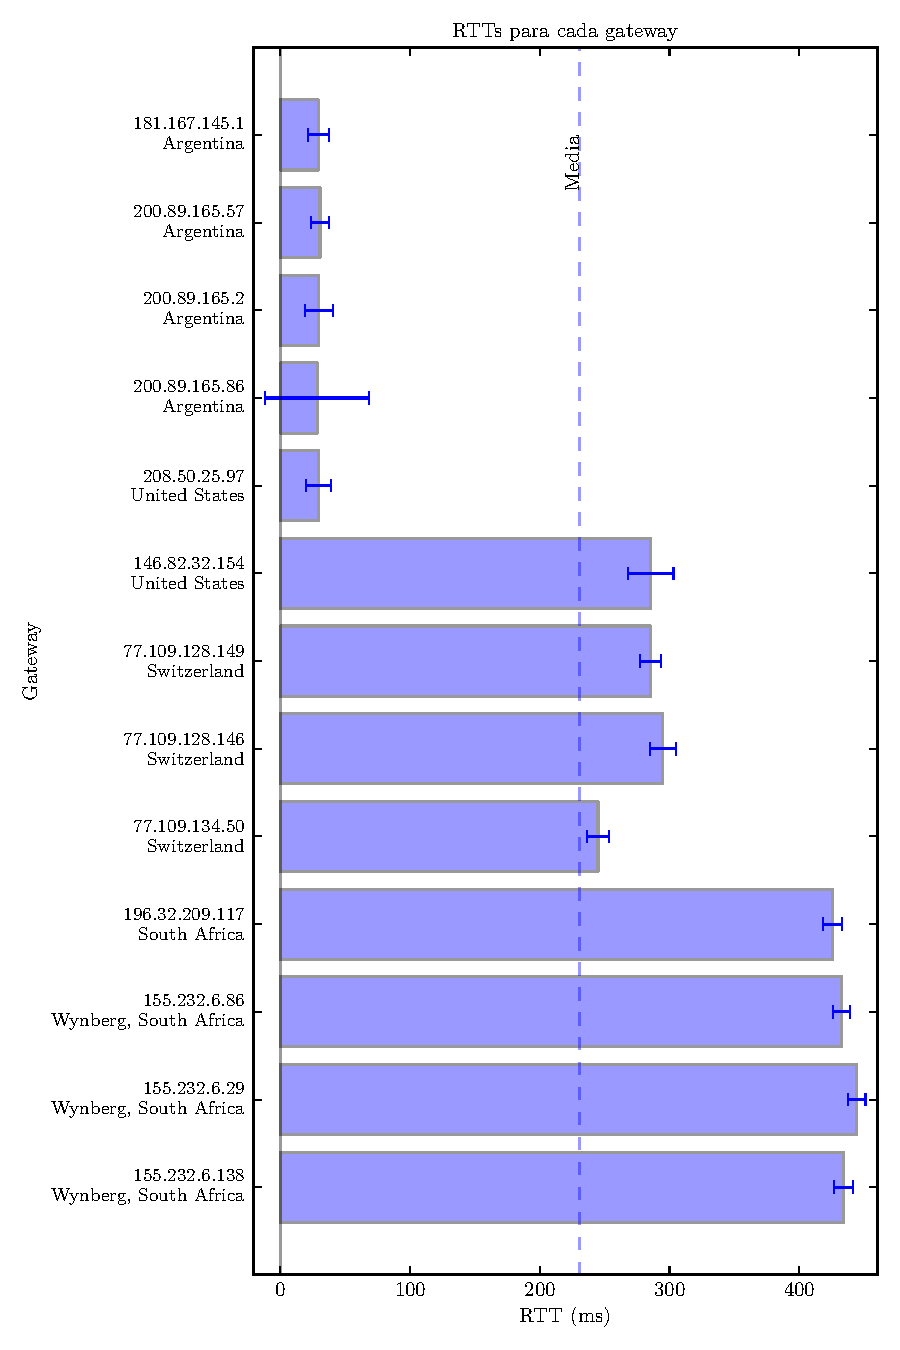
\includepdf[scale=0.70]{../imgs/rtt-unisa.pdf}
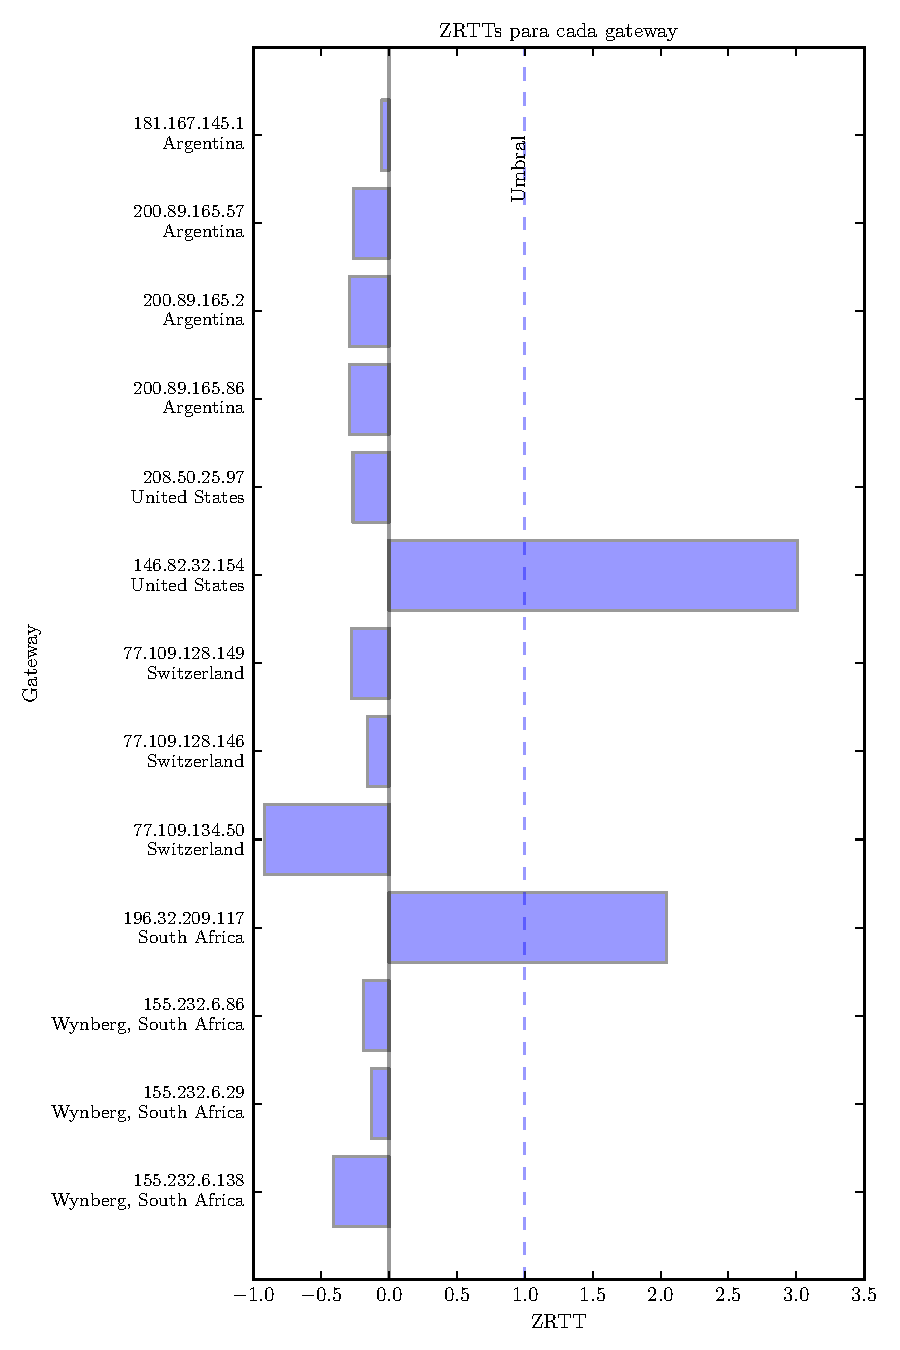
\includepdf[scale=0.70]{../imgs/zrtt-unisa.pdf}

\subsection{University of Zurich}
\begin{figure}[H] %[h] Aqui [b] para button [t] para top
\begin{center}
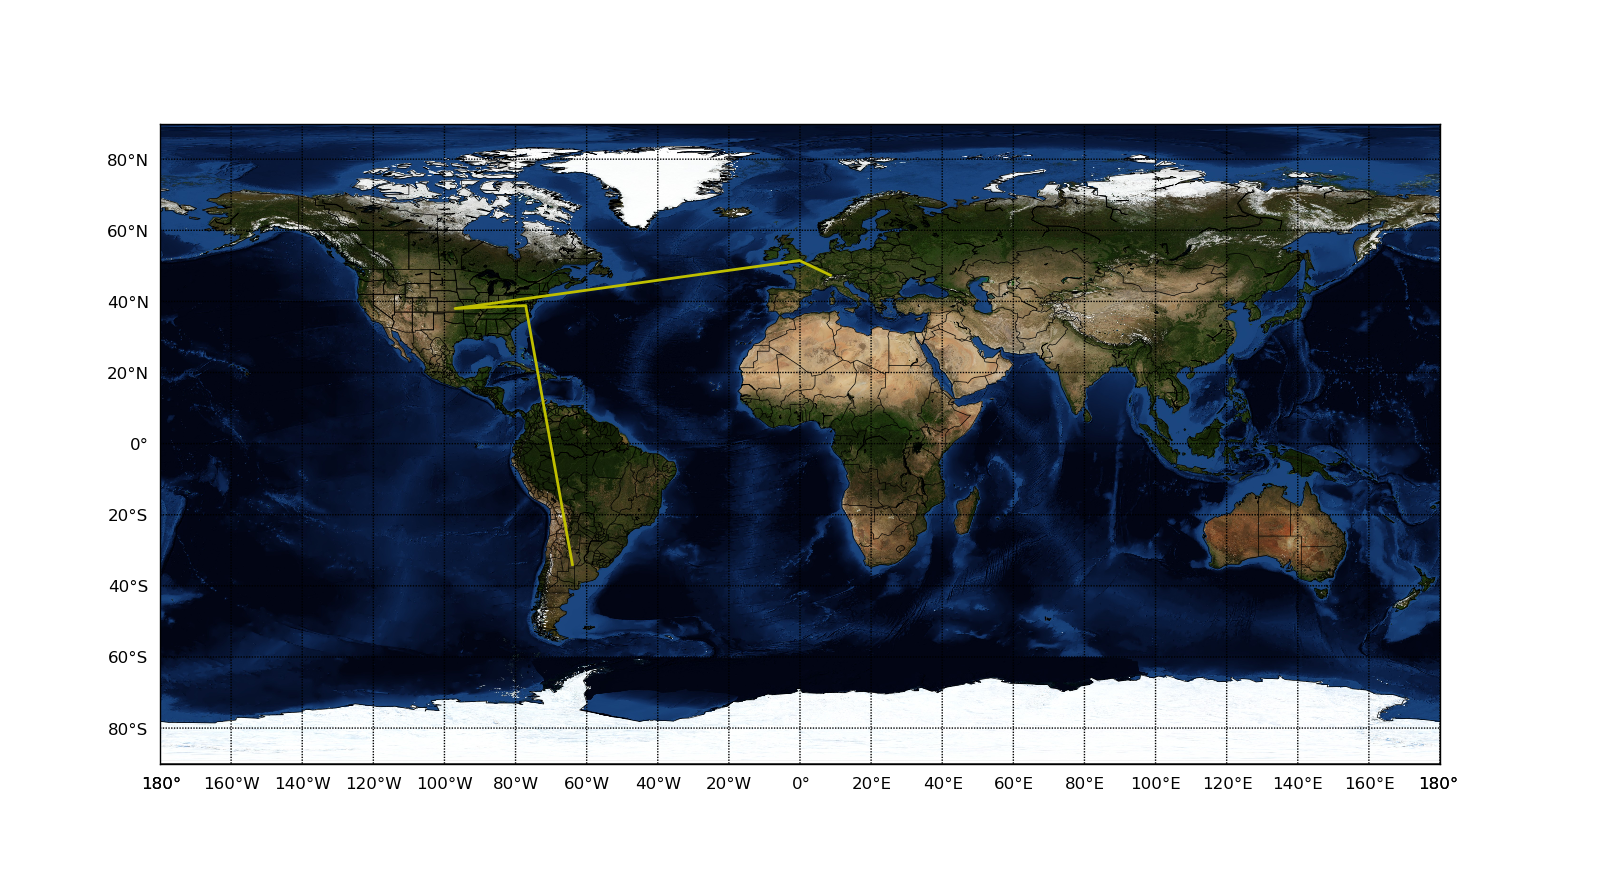
\includegraphics[width=400pt]{../imgs/map-uzh.png}
\caption{Ruta hacia University of Zurich desde servicio Fibertel.}
\end{center}
\end{figure}

\begin{figure}[H] %[h] Aqui [b] para button [t] para top
\begin{center}
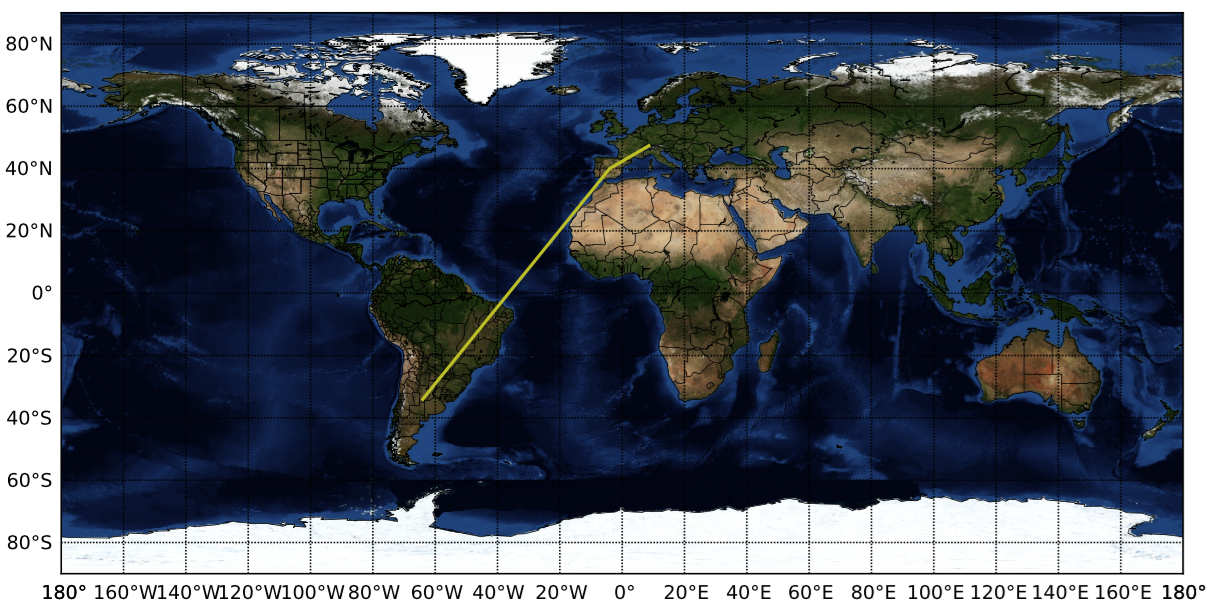
\includegraphics[width=400pt]{../imgs/map-uzh(telef).png}
\caption{Ruta hacia University of Zurich desde servicio Telefónica.}
\end{center}
\end{figure}

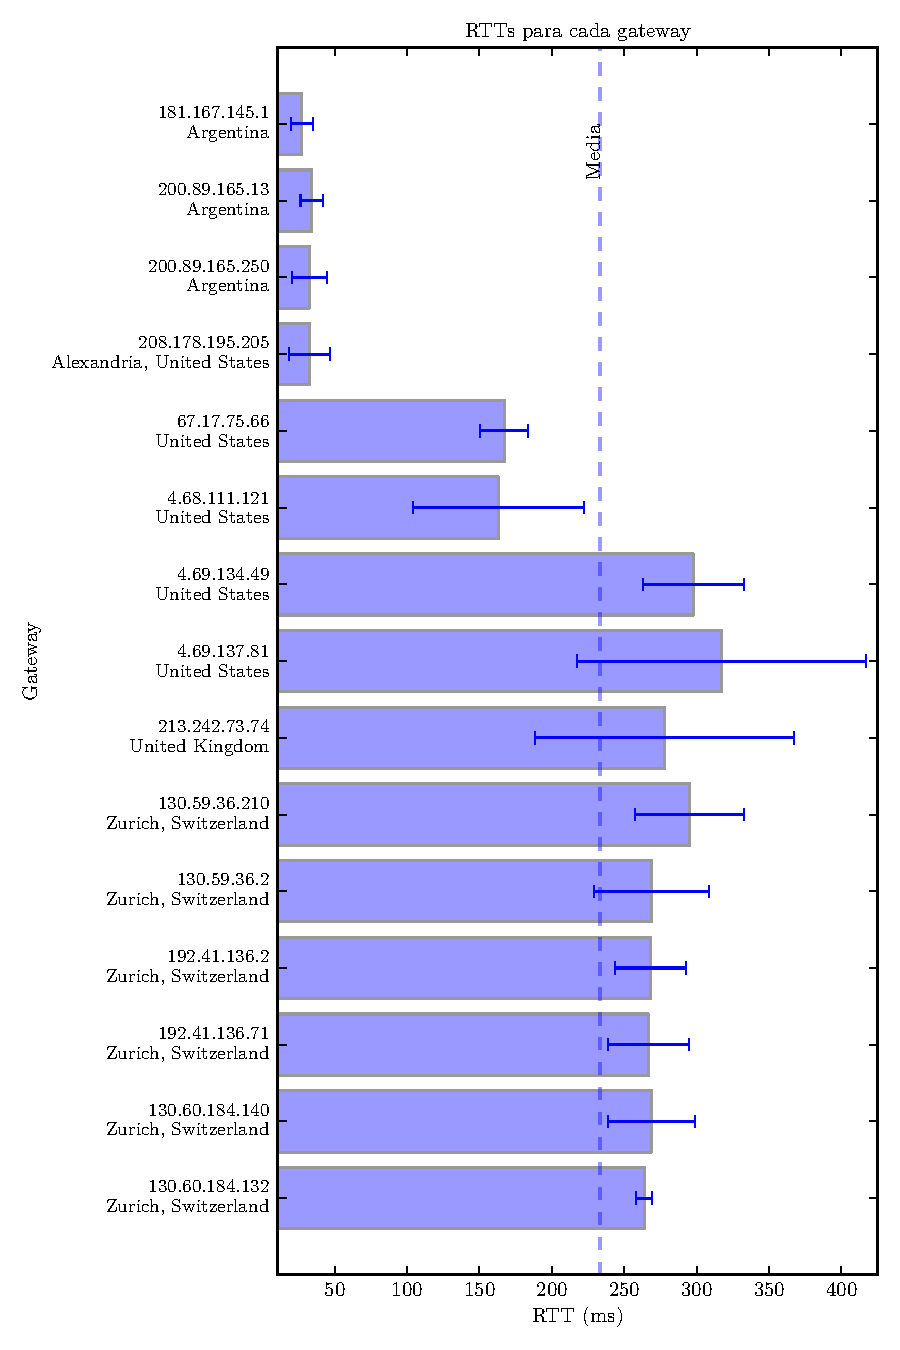
\includepdf[scale=0.70]{../imgs/rtt-uzh.pdf}
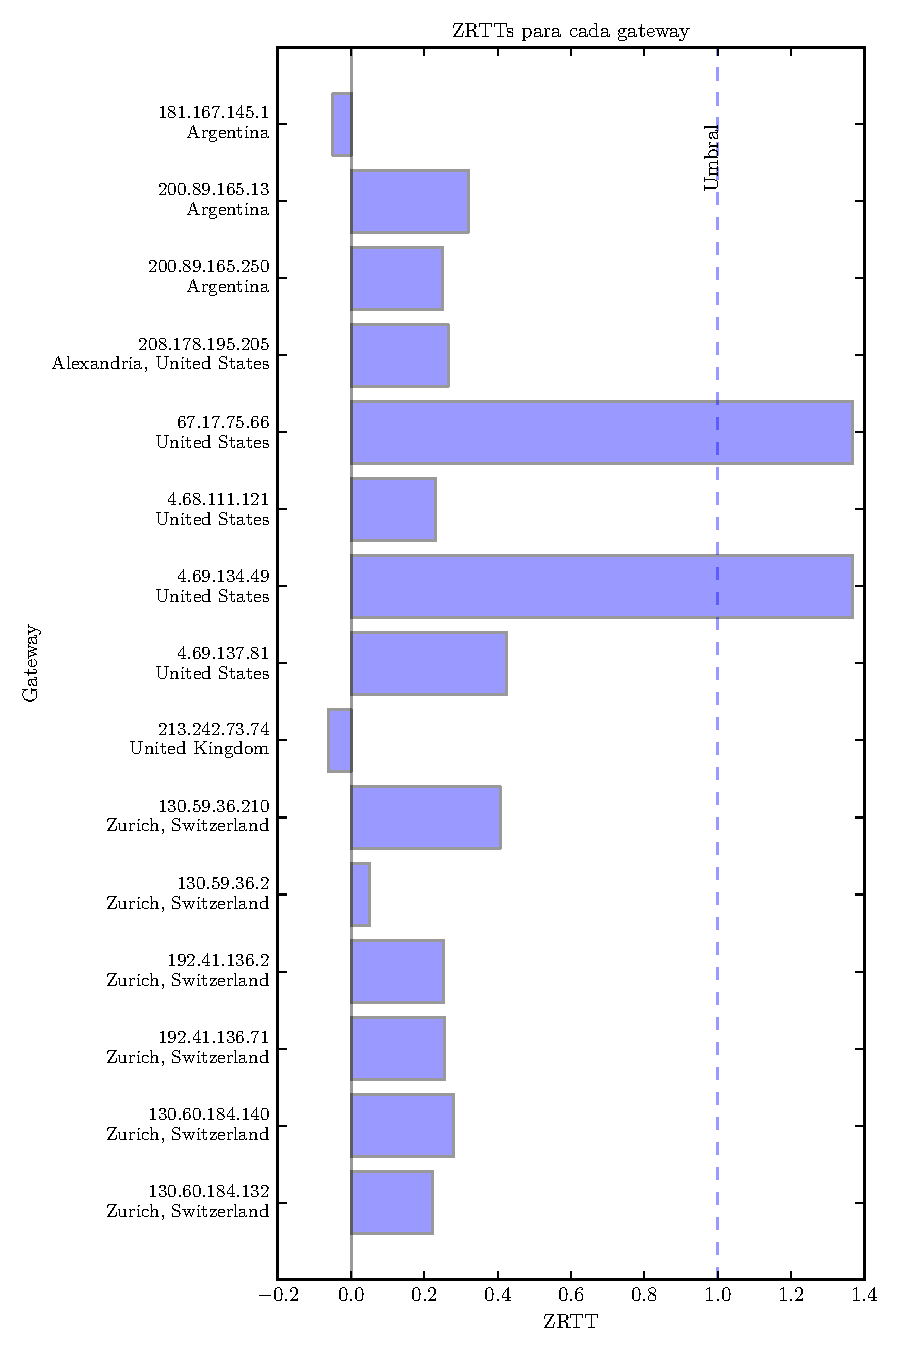
\includepdf[scale=0.70]{../imgs/zrtt-uzh.pdf}
\subsection{International University of Japan}
\begin{figure}[H] %[h] Aqui [b] para button [t] para top
\begin{center}
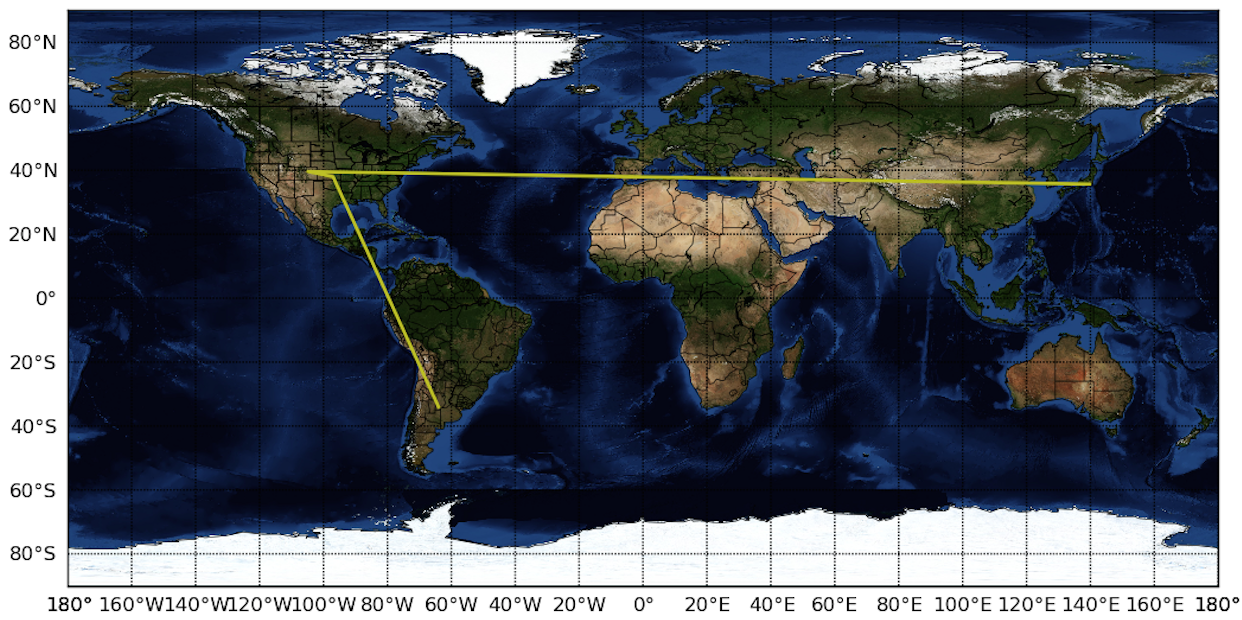
\includegraphics[width=400pt]{../imgs/map-iuj.png}
\caption{Ruta hacia University of Japan desde servicio Fibertel.}
\end{center}
\end{figure}

\begin{figure}[H] %[h] Aqui [b] para button [t] para top
\begin{center}
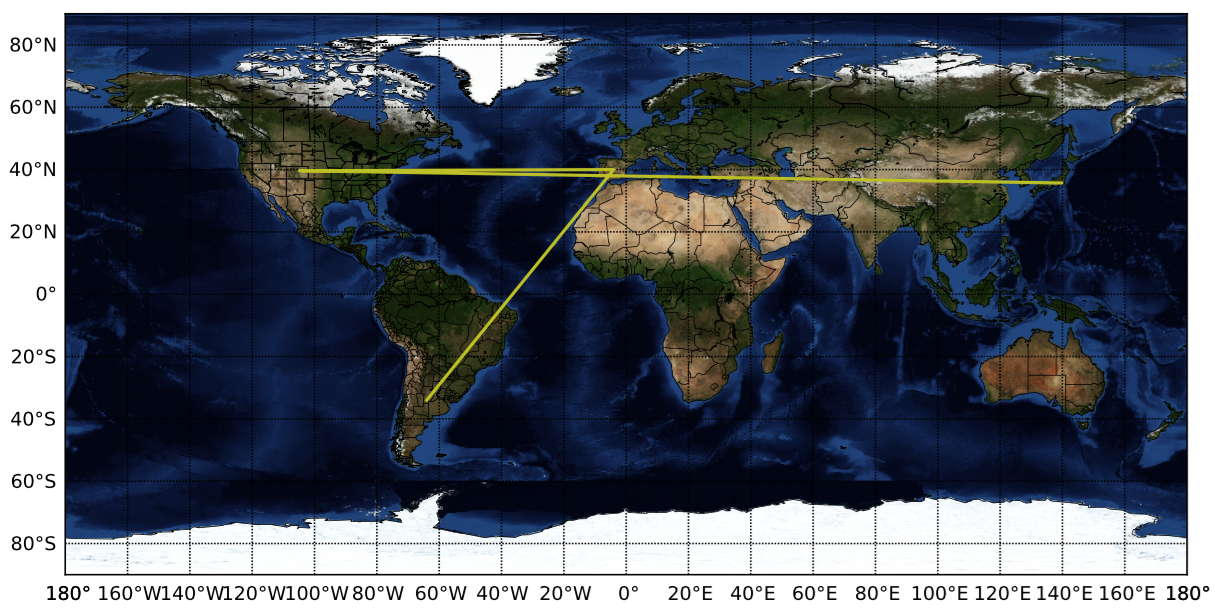
\includegraphics[width=400pt]{../imgs/map-iuj(telef).png}
\caption{Ruta hacia University of Japan desde servicio Telefónica.}
\end{center}
\end{figure}

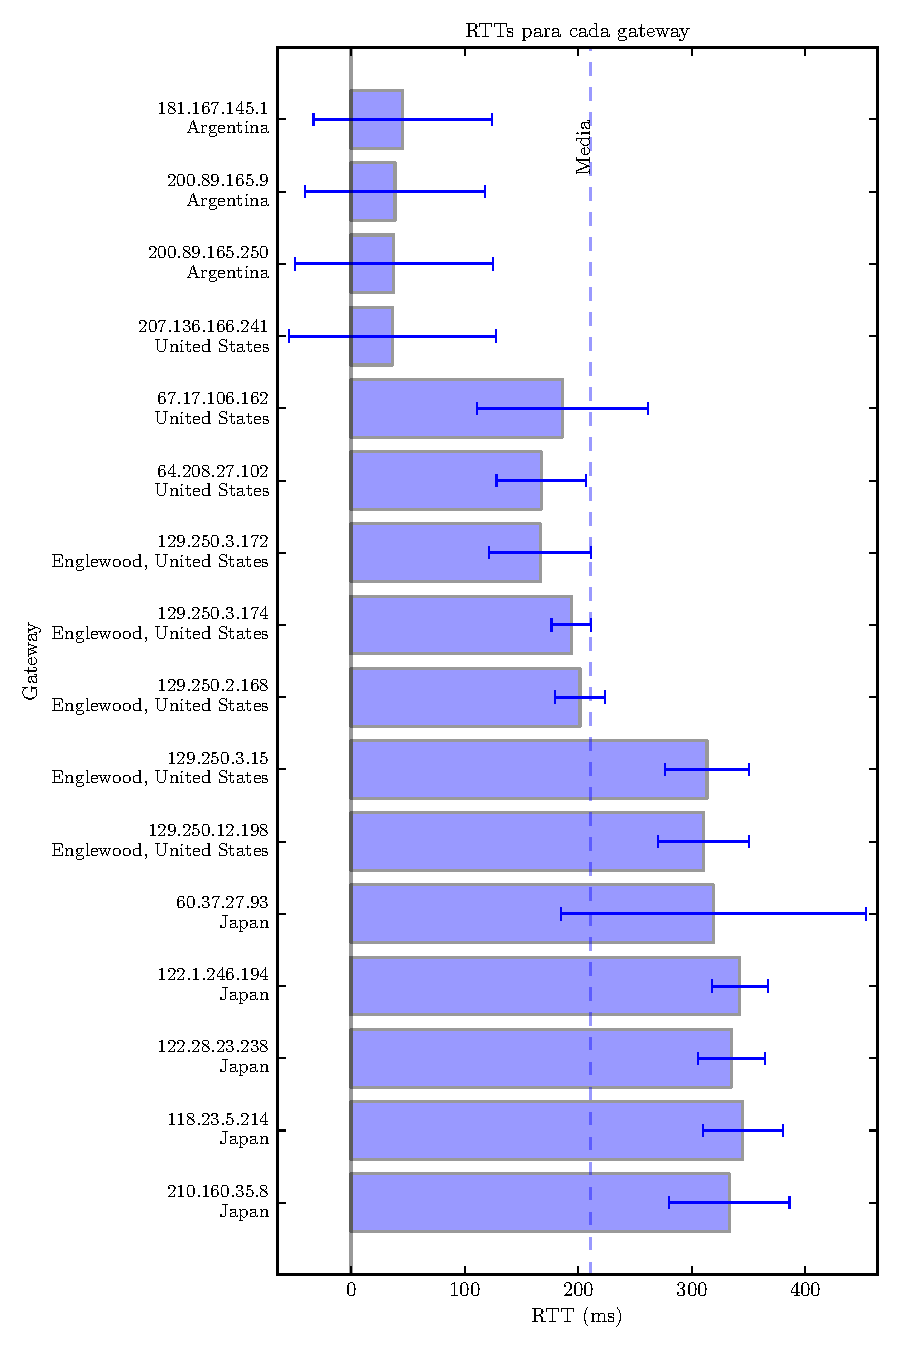
\includepdf[scale=0.70]{../imgs/rtt-iuj.pdf}

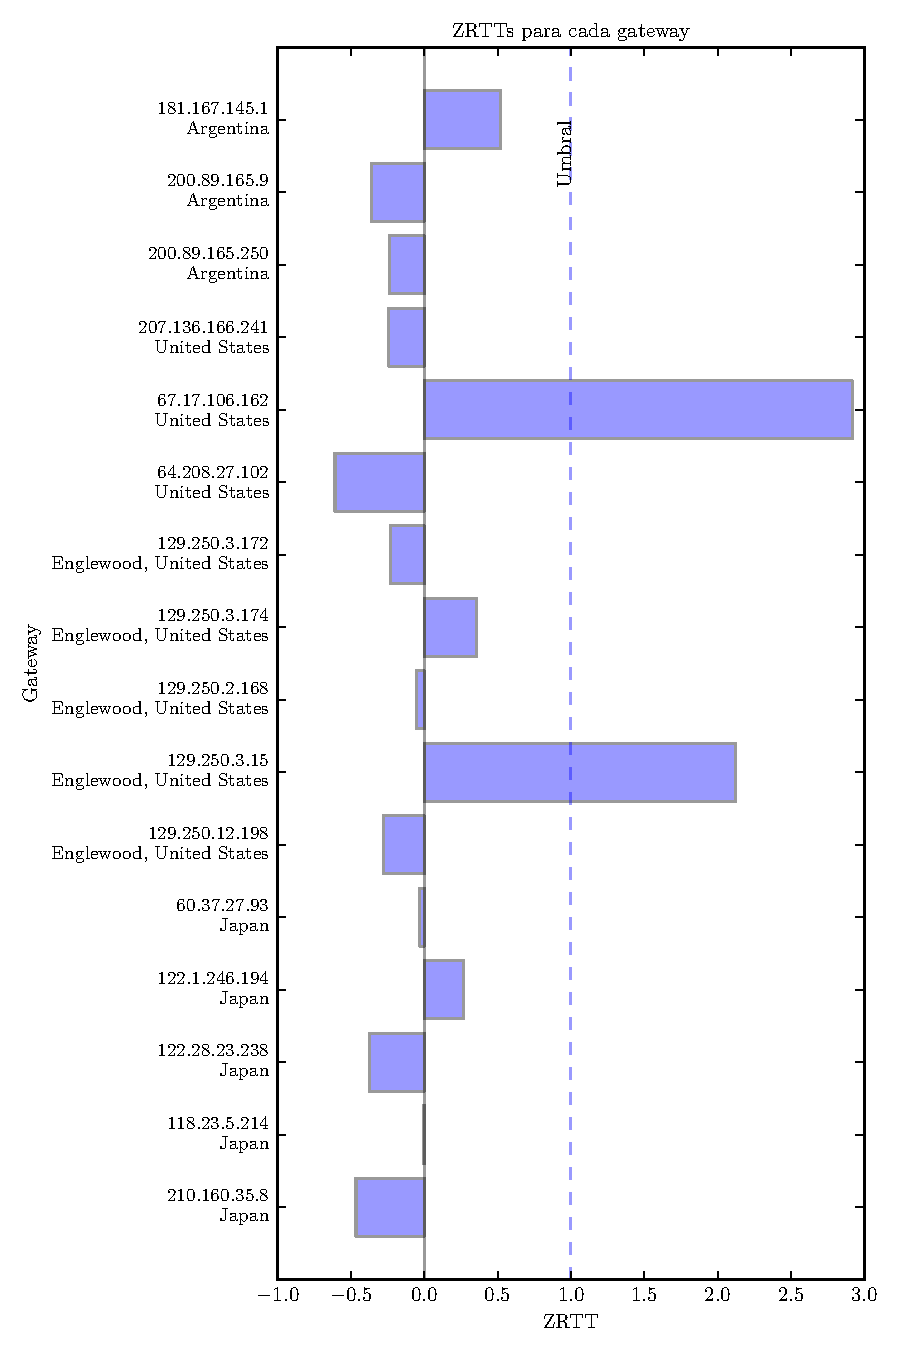
\includepdf[scale=0.70]{../imgs/zrtt-iuj.pdf}
\newpage
\section{Discusión}
Dados los gráficos presentados en la sección anterior, pudimos hallar distintos resultados. 

En primer lugar, encontramos posibles errores del geolocalizador utilizado para las IPs. Por ejemplo, al notar que todas las rutas del gateway de \textbf{Telefónica} pasan siempre por España, creemos que seguramente la empresa que provee los enlaces transatlánticos tenga IPs reservadas y, dado que se encuentra registrada en España, el geolocalizador le asigna dicha localización. Esta falla se puede ver en la latencia de los saltos dado que en algunos casos, como \textbf{University of Japan}, no tiene sentido que la latencia de Argentina a Estados Unidos sea menor que la de un vínculo interno entre Argentina, siendo este último el lugar de origen.

Por otro lado, encontramos como anómalo obtener, para un determinado nodo, un RTT absoluto menor al RTT absoluto del nodo anterior, lo que significaría que llegar a este nodo toma menos tiempo que llegar al anterior. Esta anomalía se debe a que los valores del RTT absolutos se calculan mediante el promedio de los RTT obtenidos para cada nodo, pudiendo el paquete ICMP haber tomado caminos diferentes y habiendo conseguido llegar de manera apenas más rápida en promedio.

\subsection{Saltos correspondientes a enlaces submarinos}

En primer lugar, basándonos en el análisis realizado sobre la experimentación, propusimos como umbral en las mediciones de los ZRTT relativos para la detección de enlaces sumbarinos el valor 1. Dicho valor nos pareció suficiente para detectar grandes variaciones en relación al desvío estándar de RTT entre nodos.

Los posibles enlaces submarinos son:
\begin{itemize}
\item En la traza a la universidad .......
\end{itemize}

En los distintos gráficos, podemos notar que los enlaces submarinos y los routers que asignan prioridad baja a las respuestas de paquetes ICMP muestran ambos un ZRTT alto, pero con la diferencia de que los routers que asignan una prioridad diferente hacen que el nodo siguiente tenga un ZRTT más bajo que el resto. Si bien se destacan del resto, usar únicamente un umbral positivo sobre los ZRTT presenta problemas a la hora de decidir si realmente pertenecen a un enlace submarino.

\section{Conclusiones}

Concluimos que la técnica estudiada funciona bien sólo en los casos que la traza hacia el host destino no exhibe gateways que demoran más en responder con paquetes ICMP de tipo Time Exceeded que lo que demoran en reenviar paquetes al siguiente hop en la ruta a su destino, ya que en esos casos la técnica puede producir falsos positivos.
En el caso general, esta técnica resulta adecuada para identificar hops candidatos a saltos submarinos, pero suele ser necesaria una etapa de análisis adicional para filtrar los falsos positivos dentro del conjunto de candidatos identificado, de manera de obtener un subconjunto compuesto únicamente por hops correspondientes a saltos submarinos.

\section{Referencias}
\begin{itemize}
\item PETERSON, DAVIE ; Computer Networks, 5th edition, Wiley


\end{itemize}
\end{document}
